\documentclass[sigconf]{acmart}

\usepackage{hyperref}
\usepackage{graphicx}
\graphicspath{ {images/} }
\usepackage{endfloat}
\renewcommand{\efloatseparator}{\mbox{}} % no new page between figures

\usepackage{booktabs} % For formal tables

\settopmatter{printacmref=false} % Removes citation information below abstract
\renewcommand\footnotetextcopyrightpermission[1]{} % removes footnote with conference information in first column
\pagestyle{plain} % removes running headers

\begin{document}
\title{Big Data Analytics for Municipal Waste Management}

\author{Andres Castro Benavides}
\orcid{1234-5678-9012}
\affiliation{%
  \institution{Indiana University}
  \streetaddress{107 S. Indiana Avenue}
  \city{Bloomington} 
  \state{Indiana} 
  \postcode{43017-6221}
}
\email{acastrob@iu.edu}

\author{Mani Kumar Kagita}
\affiliation{%
  \institution{Indiana University}
  \streetaddress{107 S. Indiana Avenue}
  \city{Bloomington} 
  \state{Indiana} 
  \postcode{43017-6221}
}
\email{mkagita@iu.edu}
% The default list of authors is too long for headers}
\renewcommand{\shortauthors}{A. Castro et al.}

\begin{abstract}
Waste management is becoming a greater concern for cities and municipalities around the world because of the continual increase in  population and waste. Big data analysis has the potential to not only help assess the current waste management strategies but also provide information that can be used to optimize the systems used in various institutions, local governments, and companies, among others.
\end{abstract}

\keywords{Municipal Solid Waste Management, Big Data, Local Government, HID305, HID319}

\maketitle

\section{Introduction}

In the current fast-paced society,  production of goods continues to increase, and new distribution chains continuously change. The generation of waste and the deprecated goods -from now on referred to as solid waste- has increased over the past ten years, rising from approximately 0.64 kg per person per day of solid waste to approximately 1.2 kg per person per day.  Projections estimate that this number is expected to increase to about 1.42 kg by 2025 ~\cite{hoornweg2012}. This continual change and increase make waste management a more complex and more intensive endeavor.  

While the quantity of waste itself can and should be reduced by conscious use and a discipline in recycling and reusing items, there is much that can be done to reduce waste in the actual collection and disposal by optimizing waste management systems.

Because of this, different local governments and organizations have recognized the need to develop more elaborate regulations to control the different features, segments, processes involved in waste disposal from the moment the material is discarded by the consumer to the moment the material reaches its ultimate destination, such as a recycling plant or landfill. This set of systematic regulations is called solid waste management. Solid waste management has changed over time.  What used to be systems designed and implemented based on local needs and convenient disposal as moved into extensively researched and implemented management systems that consider complex multivariate and dynamic sources of data ~\cite{akbarpour2016}.

Currently, data used in waste management is collected from many sources and varies depending on the types of solid waste and the rate of disposal. Because of the diversity of sources available (including types of waste, weight collected, the location of collection and disposal, etc.), the quality of the data must be continually monitored and assessed ~\cite{chandrappa2012}. New management systems that seek to optimize waste management must collect large volumes of data from each data source on a daily basis. Multivariate data analysis methods provide exploratory data analysis, classification and parameter prediction using this data ~\cite{bohm2013}.

\section{ Municipal Solid Waste Management}
%a) what is the problem

There are significant differences between the general composition of the waste generated in rural areas and the waste produced in urban areas. The waste produced in the later is profoundly influenced by the culture and the practices of our modern society.  This distinction means that there will inevitably need to be differentiation in waste management practices and systems based on each communities needs, commerce, economy, and practices ~\cite{chandrappa2012}.

Municipal Solid Waste (MSW), commonly known as garbage or trash, consists of items that residential, commercial, institutional and industrial sites generate. This is much different from the type of waste produced, for example, in an agricultural community.  Urban, or municipal, waste can be the result of everyday activities, such as leftover food, plastic bottles, packaging material, wooden furniture, electrical and electronic appliances, glass, medical waste, cardboards, waste tires, office wastes, consumer goods, among others. 

The amounts of solid waste and its composition vary depending on the country, place, and activity performed at the site where the waste is generated ~\cite{chandrappa2012}. For this reason, every process related to waste management-transportation, storing and final disposition, among others- must be engineered and tailored to fit the specific needs of community, organization, or local institution.  The data collected for analysis will also be specific to the needs and realities of each individual entity, which is why waste management plans are not universal or easily applied from one community to another.  

The ways of handling waste have also changed over the years, affecting the best ways to manage waste. According to EPA statistics from 2014, Americans have generated about 258 million tons of MSW of which more than 89 million tons is recycled and composted. The equivalent to a 34.6\% recycling rate compared to 6.4\% in 1960. Americans have also used the energy production process to combust approximately 33 million tons of waste,  while as much as 136 million tons of waste ended up in landfills during the same year ~\cite{epa2014}.  Because of this, data on recyclable material, dividing waste and recyclable material, and where materials are sent or how they are disposed of has also become significant. Figures 1,2,3 and 4 ~\cite{epa2014} represents MSW generation rates, recycling, composition rates and Total MSW generation between 1960 and 2014 ~\cite{epa2014}.

\begin{figure}[ht!]
  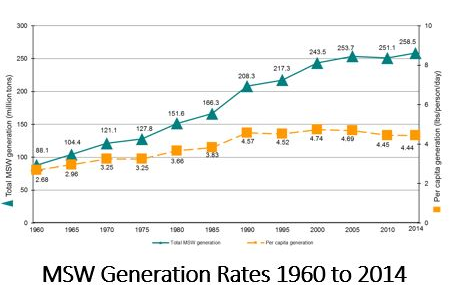
\includegraphics[width=0.5\textwidth]{fig1.png}
  \caption{MSW Generation Rates in US from 1960 to 2014}
\end{figure}

\begin{figure}[ht!]
 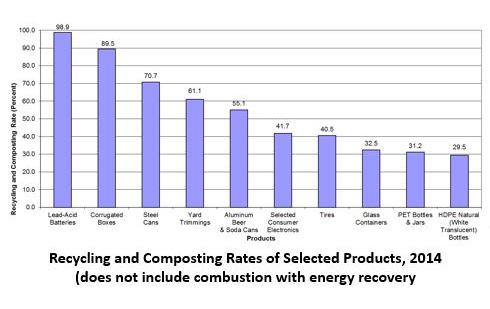
\includegraphics[width=0.5\textwidth]{fig2.png}
 \caption{Recycling and Composting Rates of Selected products in US, 2014}
\end{figure}

\begin{figure}[ht!]
  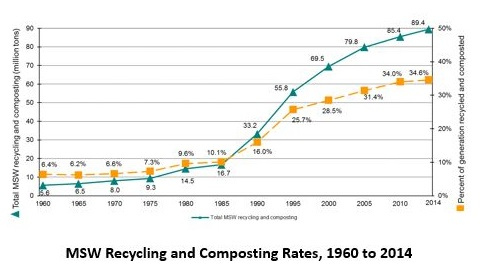
\includegraphics[width=0.5\textwidth]{fig3.jpg}
  \caption{MSW Recycling and Composting Rates in US from 1960 to 2014}
\end{figure}

\begin{figure}[ht!]
  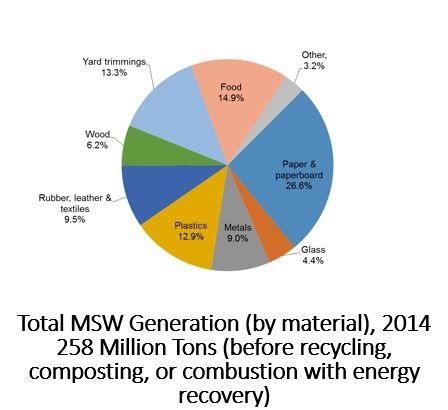
\includegraphics[width=0.5\textwidth]{fig4.jpg}
  \caption{Total MSW generation in US, 2014}
\end{figure} 

In waste management, decision-makers are and will continue to be forced to make choices.  When they develop or implement plans, they have a choice as to what information they will or will not consider for analysis.  They have to choose what factors are influential in their jurisdiction.  They make choices about routes, resources, and all the details between pick up to disposal.  These choices can be classified as fortuitous, good, or optimal ~\cite{akbarpour2016}.

Fortuitous decision-making has no scientific base; the person who is in charge of making decisions must always try to solve the problem with little or no research or data.   On the other hand, good decision-making is primarily based on experience, comparison of elements and trial and error.  Optimal decision making, however, requires understanding and analysis of techniques and technologies provided by other fields ~\cite{akbarpour2016}.

This is where Big Data comes in. 

\section{ Big data and waste management}
%b) why is big data involved

Big data has the capacity to facilitate analysis of information so that better decisions can be made.

In Big Data, the expert in charge takes many data sets coming from diverse and dynamic data sources and applies technologies to analyze these data sets.  Authors of papers and books like ''The Fourth Paradigm'' state that big data exploration works to find patterns in data by analyzing the trends and outliers found in the datasets mentioned above, to generate knowledge ~\cite{hey2009fourth}.

Characteristics (such as the large volume of data generated in waste management, how dynamically the data is generated, and the variety of formats in which the data comes) turn the task of producing knowledge an ideal task for Big Data.  Scientists can interpret the findings of Big Data  in a way that allows individuals and institutions involved in waste management, to make optimal decisions ~\cite{yenkar2014review}. 

By using Big data, local governments can also track the number and quantity or weight of disposals at different locations; this information can be mapped to reveal the locations of the most significant waste generators.  This information will help entities develop specific strategies to reduce waste and help implement permanent solutions for better environments ~\cite{markvan2016}.

\subsection{ Examples of Big data and waste management}

In Manchester, England, the Greater Manchester Waste Disposal Authority, England's most significant waste management institution, has started to use Big Data to better orchestrate the waste management services they provide. To get the most out of their Big Data approach, the Greater Manchester Waste Disposal Authority is working in collaboration with the research done by the University of Manchester. Together, they are creating environmentally sustainable solutions for Manchester, and are finding optimal solutions to the 1.1 million tonnes of waste that Manchester produces every year ~\cite{markvan2016}. 

Another example of a local government implementing Big Data Solutions is the city of  Songdo, South Korea. In said city, every citizen needs to use a chip card while disposing of their garbage. Data collected from these chip cards is being used to analyzing on the quantity of disposed waste and their locations. Each trash bin is incorporated with sensors to provide the height of the garbage accumulated in the reciprocal, temperature, and air pollution levels. These multiple parameters help municipal authorities forecast ideal times to collect the trash and optimize the routes to save time and expenses ~\cite{markvan2016}.

Researchers in Ethiopia are combining socioeconomic data alongside geographic data in order to get a clearer understanding of the patterns of how household waste is being collected and distributed. This study helped local authorities to better manage waste practices in urban areas ~\cite{markvan2016}. 

A group of researchers from the University of Stockholm is using Big Data to identify how to optimize waste management routes in their city. By using a wide variety of data sets collected from various sources, roughly around half a million entries including trash bin locations, weights, and truck routes, researchers have developed waste generation maps of Stockholm. This research has helped reveal various inefficiencies in the current waste management system and will be integral in helping them improve their local waste management ~\cite{markvan2016}.
Figure 5 ~\cite{shahrokni2014big} represents heatmap of all waste aggregated per zip code in Stockholm.


\begin{figure}[ht!]
  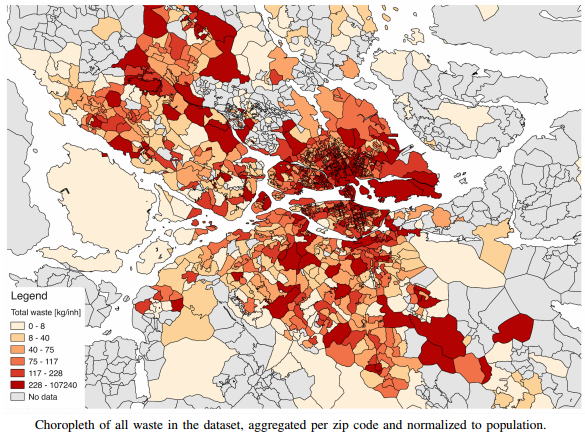
\includegraphics[width=0.5\textwidth]{stockholm.png}
  \caption{Choropleth of all waste, aggregated per zip code and normalized to population in Stockholm}
\end{figure}

\subsubsection{Vehicle Routing Problem}
Vehicle route optimization is one of the primary concerns in waste management. It is termed as Vehicle Routing Problem (VRP) ~\cite{dantzig1959}.   While routes may be designed based on geography, merely looking at a map and designing what seems to be practical movement through the city, this is underestimating the extent of the factors involved.  There are multiple factors that either directly or indirectly affect waste collection that can also be analyzed and considered while designing routes. Common known factors that influence vehicle routing are the type of vehicle, vehicle capacity, number of collection stops, volume per capita and the route length. Figure 6 represents Vehicle Routing Problem ~\cite{wikivrp2017} when one dump location is placed between different collection routes.

\begin{figure}[ht!]
  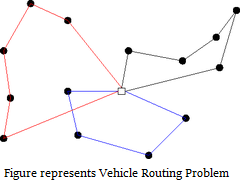
\includegraphics[width=0.5\textwidth]{vrp.png}
  \caption{Vehicle Routing Problem}
\end{figure}

Two of the most basic VRPs are the Travelling Salesman Problem (TSP) and the Chinese Postman Problem (CPP) ~\cite{belien2012}. However, when too many constraints and attributes are considered, both of the TSP and CPP become more difficult problems to solve. Many researchers have studied and published articles on waste management vehicle routing problemVRPs, and yet it is a persistent problem. Mathematical models need to be developed to provide city administrators with tools to make effective long-and short-term decisions relating to their municipal disposal system ~\cite{bhat1996}. 

In addition to the common known factors causing VRP problems, indirect attributes must also be taken into consideration.  Time of day, traffic, weather patterns, energy prices, demand fluctuations, vehicle health, dump site inventory also have potential to affect route efficiency. 

A research team at OSI came up with a better solution for solving VRP problems using Big Data technologies. Mixed Integer Programming (MIP) formulation was designed to interact with millions of attributes in live environments providing real-time decisions to optimize the VRP. Big Data technologies are being used to enable prediction of travel times and forecast and address demand on a tactical timeline. This approach has helped improve VRP forecasting between  5\% to 10\% ~\cite{vijay2013}. Any improvement, even less than 5\% created on VRP is a significant improvement ~\cite{hasle2007}.

Scientists and engineers have designed a system that communicates between waste reciprocals, waste collection vehicles and a central system using sensors that measure how full containers are and can send real-time data ~\cite{faccio2011}.

The data collected can be used to optimize routes and space in the waste collection vehicles.  Sensors can identify which containers do not need to be collected, allowing them to shorten routes.  In addition, sensors can measure the remaining capacity of collection vehicles, allowing them to extend routes when they still have cargo space, ensuring that they return to the disposal center only when they are carrying a full load.  By using these sensors, fewer collection vehicles were needed.  It was estimated that in three years, the expense of purchasing and implementing this system would be recovered ~\cite{shahrokni2014big}.

In addition to the real-time data collection that helps optimize collection and routes, remote self-diagnostics are also helping optimize vehicle use.  By being able to monitor the vehicles use and health, maintenance and repair are more efficiently managed.  Through this system, managers are made aware of parts that need to be ordered in advance, limiting the time that the vehicles may be out of service.  Handheld devices have been developed for service verification, further helping minimize external providers or assessments, optimizing asset management and costs ~\cite{megan2017}.


\subsubsection{Problem of Landfill Disposal}

A municipal solid waste landfill (MSWLF) is a individually separated area of land or a trench where the household waste is collected and stored. These landfills are designed to store municipal solid waste as well as other wastes like construction and industrial waste. These landfills can be open-pits or below ground refuse chambers. In recent years, its becoming more expensive to operate and maintain these landfills as to protect the environment from escaping liquid pollutants and causing water and surface contamination. These liquid pollutants are commonly called as Leachate. It forms when water originating from rainfall or groundwater dissolves gradually through a porous surface and dissolves the chemicals from the refuse especially if the protective layer of the landfill allows liquid or gases to pass through it. 

Leachate contamination problems became more problematic in older landfill sites when they are typically lacked in barriers above or below the landfills which causing pollution and diseases to the citizens residing in areas near to these landfills. In modern days, Governments across the world are in one motive to prevent waste disposal and reduce landfill deposits. Steps are taken to reduce number of landfill areas and extending landfill capacity at current sites. Figure 7 displays the number of landfills in the US, 2009.

\begin{figure}[ht!]
  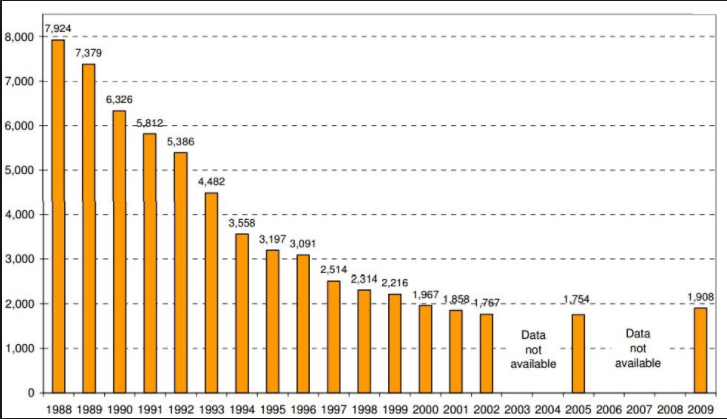
\includegraphics[width=0.5\textwidth]{landfills.png}
  \caption{Number of Landfills in the US 1988-2009}
\end{figure}

Landfill disposal, in itself, has its own set of complex factors including measurement and control of gases, management of waste water, and precipitation patterns affecting water volume in the geological basin.  

Identifying these factors creates an opportunity to develop sensors that could collect meaningful data that would be an asset to optimizing landfill disposal.  Sensors could measure gas emission, water volume in disposed waste, and precipitation.  Having this information would allow data scientists to develop systems that would identify when disposal would need to be varied, how water treatment plants could efficiently manage runoff and basin water and communicate with water treatment plants to use more or less of their mechanical resources based on real-time needs. 

Manual calculation would be time-consuming and physical observation opens space for inefficiency and delay.  In order to compute these calculations promptly so that the information could contribute to optimization, it would be ideal to develop a computer program to compute the mathematical operations.  This would contribute significantly to optimization of water treatment, for example, in landfill disposal ~\cite{akbarpour2016}.

Waste management is already in the process of transforming from using older methodologies to modern Big Data technologies. Big Data has a lot more potential to eradicate most of the problems faced by government in waste disposal. Most of the government organizations are taking a leap to minimize disposal of waste and to achieve "zero waste" ~\cite{rosengren2017} goals. A program in government of District of Columbia called "Zero Waste DC" is being initiated to develop and provide resources that will help its residents move towards zero waste. Its main motive is to divert 80\% of MSW to recycling or source of energy where the remaining 20\% non recoverable waste will be sent to landfills. By collecting vast amounts of data from all sources, they will analyze it to implement cost-effective strategies for converting waste to re-usable resources, improving environmental conditions, taking measures on human health, reducing greenhouse gas emissions and conservation of natural resources. Obtaining data from the sensors on contamination of air with harmful gases, water purification levels from the nearby lakes, physical properties as well as chemical properties of the soil, Big Data will help to analyze this data and provide solutions to prevent them from making situations worst ~\cite{rosengren2017}.

When its considered Big Data as a volume, huge amounts of data is being collected daily from different sources like digital meters, sensors, social media to avoid waste disposals. It is how this data is being turned into knowledge to apply into real-world problems. Cloud based solutions and using IoT sensors becoming more insight technologies for smart cities and municipal waste management authorities to optimize the waste and their recycle operations. Big Data will help in lowering of contamination on the waste and improve consumption habits of residents in urban areas.

Reading information from the sensors placed in recycle bins, it is easier to figure out what type of waste is being disposed in the trash bins and by which resident. If there are hazardous materials located, authorities can detect them before even being collected by the trash collectors. This will help to educate corresponding resident on the importance of waste and their contamination results. Big Data Analysis encourage citizens to understand about food scraps so that it can be reused as fertilizer for many of the organic foods. It is termed as "farm to farm" practice according to Robert Reed, Evangelist at Recology ~\cite{james2012}.

Using Big Data technology to collect real-time data thought the waste disposal process especially for food wastage allows visibility to organic waste. This shows focus on identifying inefficiencies in food management process which in turn helping them to initial improvement in process and to create immediate effects. Optimizing waste management is a key to find operational efficiencies and to support environmental directives. It enables business to make effective decisions about purchasing or production of organic waste ~\cite{frank2016}.

Environmental Protection Agency US also using benefits of Big Data in recycling of waste. Big Data Analysis helps in identifying quantities of solid waste being recycled and assessing the residents on the benefits they receive by recycling achievements. MSW Characterization Report shows the data collected on generation and disposal of waste in US past 30 years. This data is being analyzed to measure waste reduction and plan recycling programs across the country ~\cite{epaRecycleBenefits2007}.


\subsection{Statistics and Waste Management}

Statistics help develop mathematical models to predict behavior based on the data collected.  In waste management, these statistics can be used by Big Data professionals to draw conclusions and foresee possible outcomes as related to effective policy making and actual waste production, collection, and disposal patterns. 

There are many data analysis methods that are used when studying waste management, but the two most popular are Principal Component Analysis (PCA) and Partial Least Squares (PLS1) ~\cite{bohm2013}. Hidden variations inside huge data sets are being displayed using PCA. Applying PCA to various fields in waste management help to find and capture relative parameters from large data sets so as to define which parameters are most significant in providing effective decision making results for waste management problems. This approach will generate results to save time and money in future research activities. PSL1 is used to calculate the principal components of external correlation between two given data matrices separately and to design and develop a regression model between the inner correlation and scores of the principal components ~\cite{bohm2013}.

Lingo is a mathematical modeling language designed particularly for formulating and solving a wide variety of optimization problems including linear programming. Lingo optimization software uses the branch and bound methods to solve problems of this type ~\cite{akbarpour2016}.  

These resources are valuable to the continual analysis of data being collected, continually helping in waste management optimization.

\subsection{GIS Analytics}

When it comes to Geographical Information Systems (From now on GIS), there are multiple software and hardware options in the market. From paid software like ArcGIS to Open and free software like GVSIG, some solutions can help interpret large data sets, apply statistics and algorithms of different kinds and display them in a way that refers to a geographical space. 

Two optimal routing algorithms have been used to calculate routes for waste collection; Solomon's insertion algorithm and a clustering algorithm.  Data was used to help create more efficient routes by minimizing driving distance while taking into consideration factors like lunch breaks (time windows) that affected the distribution of human resources and time/vehicle management.  By adding vehicle depots, by rerouting, and by sharing various routes, they predicted that they would be able to shorten vehicle expenditure by as much as 10,000 km.  

An additional routing algorithm was used to present information on the environmental significance for optimizing waste collection routes.  The study assessed the use of roll-on/roll-off containers while also considering schedules and lunch breaks.  Through the utilization of an adaptive large neighborhood search algorithm, alongside a clustering method, a residential waste collection was analyzed, taking into consideration actual pick up points and employee lunch breaks.  Using this information, time windows and starting conditions were adapted alongside the routes to reduce the total distance by as much as forty-five percent ~\cite{shahrokni2014big}.

\section{Conclusion}
Waste management has been a growing concern and will continue to be an important area for optimization as both consumer waste and population increase.  As institutions, governments, and individuals look to assess and optimize resources, minimize cost and create less of an environmental impact of waste management, Big Data has the potential to continue to help provide the information needed for future advancement.

There are various tools being used to optimize the different waste management practices, and there is space to develop additional tools to continue to the information available to decision makers.

One of the main reasons to use Big data in Municipal Waste Management is to provide local governments with tools that would facilitate the implementation of systems to more efficiently manage how much, where and the growth rate of the material that the community dispossess. Optimizing the waste management systems can help minimize the environmental impact of the community's actions, reduce pollution, increase rates of recycled materials, optimize routes to reduce time and expenses, among others.
 
Waste Management is not only government issue. Citizens should take the initiative and educate others on how to recycle and reduce waste. With the help of the collected data, governments can notify the different entities (individuals, communities, companies and other organizations) a equip them through education and awareness, and also share valuable information about the importance of waste management through different media, such as mobile phones, email, among others.

Local governments have just started to adopt Big Data technologies for solving problems involved in MSW, but there is plenty of room for growth and further use and development.  By using Big Data Analytics, large amounts of data sets pertaining to specific communities waste, routes, and disposal can be used to identify trends and patterns that could highlight opportunities for improvement. Big Data can play a significant role in managing cities more efficiently, benefiting not only those managing the systems, but the communities in which they are implemented as well.

\begin{acks}

The authors would like to thank Dr. Gregor von Laszewski for his support and suggestions in writing this paper.

\end{acks}
\bibliographystyle{ACM-Reference-Format}
\bibliography{andrew} 

\end{document}
